\begin{titlepage}
 \setlength{\unitlength}{\textwidth}
  \begin{picture}(1,1.41)              % pagxforma
    \put(0.1,0.1){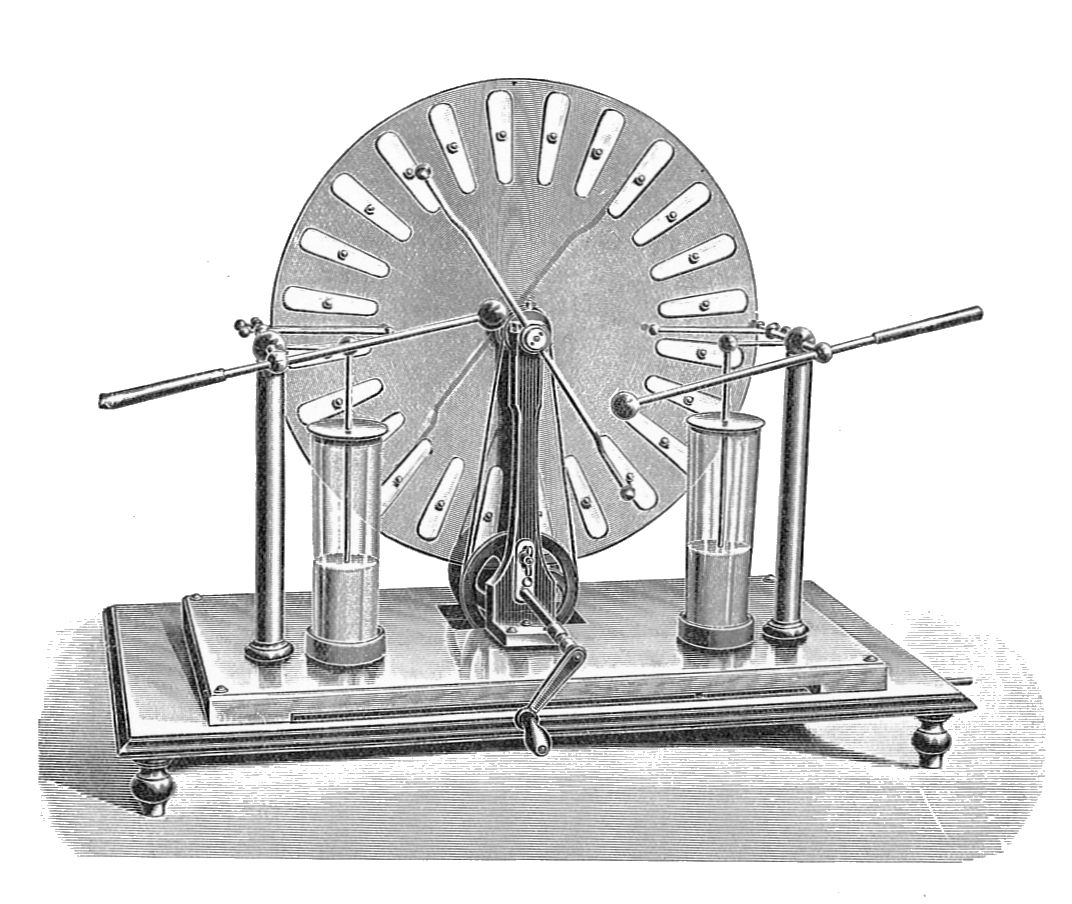
\includegraphics[width=0.8\textwidth]{Wimshurst-bw}}
    \thinlines
    \put(0.05,0.05){\line(0,1){1.31}}         % vertikala linio maldekstra
    \put(0.95,0.05){\line(0,1){1.31}}         % vertikala linio dekstra
    \put(0.05,0.05){\line(1,0){0.9}}            % horizontala linio malsupra
    \put(0.05,1.36){\line(1,0){0.9}}         % horizontala linio supra
    \thicklines
    \put(0,0){\line(0,1){1.41}}         % vertikala linio maldekstra
    \put(1,0){\line(0,1){1.41}}         % vertikala linio dekstra
    \put(0,0){\line(1,0){1}}            % horizontala linio malsupra
    \put(0,1.41){\line(1,0){1}}         % horizontala linio supra
    \put(0.5,1.2){   \makebox(0,0){\huge W.F. Hermans}}
    \put(0.3,1.1){\line(1,0){0.4}}
    \put(0.5,1.0){ \makebox(0,0){\huge La elektrilo} }
    \put(0.5,0.92){ \makebox(0,0){\Large de }}
    \put(0.5,0.84){ \makebox(0,0){\Huge Wimshurst} }

  \end{picture}
\end{titlepage}
\pagestyle{empty}
% \vspace*{\textheight}
\hbox{}
\vfill
      \begin{figure}
       \centering
        
\includegraphics[width=0.4\textwidth]{WF-Hermans}\\
        \em{W.F. Hermans}
     \end{figure}
\begin{minipage}[t]{\textwidth}
Elnederlandigo de `De elektriseermachine van Wimshurst'.  Rakonto unuafoje aperinta en la rakontaro `Een wonderkind of een total loss'
(Mirinfano a\u{u} kompleta perdo) en 1967.\\

La plej nova versio de tiu \^ci traduko \^ciam trovi\^gas je:\\
\href{http://purl.org/NET/mihxil/wimshurst/}{http://purl.org/NET/mihxil/wimshurst/}\\

\^Gi ne jam pretas!

Michiel  Meeuwissen $<$mihxil@gmail.com$>$\\

Kompostita per \LaTeX\\
Versio: \input{revisio}
\end{minipage}
\newpage
\pagestyle{plain}
\setcounter{page}{1}
